\subsection{实验目的-配置 iptables 禁止访问 ftp 服务}
通过配置 iptables 防火墙禁止访问 ftp 服务
%
\subsection{实验原理}
\begin{enumerate}
  \item Iptables 防火墙在做信息包过滤决定时,有一套遵循和组成的规则,这些规
    则存储在专用的信息包过滤表中,而这些表集成在 Linux 内核中。在信息包过滤
    表中,规则被分组放在我们所谓的链(chain)中。而 \texttt{netfilter/iptables} IP
    信息包过滤系统是一款功能强大的工具,可用于添加、编辑和移除规则。
  \item FTP 是 File Transfer Protocol(文件传输协议)的英文简称,而中文简称
    为“文传协议”。用于 Internet 上的控制文件的双向传输。同时,它也是一个
    应用程序(Application)。基于不同的操作系统有不同的 FTP 应用程序,而所
    有这些应用程序都遵守同一种协议以传输文件。在 FTP 的使用当中,用户经常遇
    到两个概念:"下载"(Download)和"上传"(Upload)。"下载"文件就是从远程
    主机拷贝文件至自己的计算机上;"上传"文件就是将文件从自己的计算机中拷贝
    至远程主机上。用 Internet 语言来说,用户可通过客户机程序向(从)远程主
    机上传(下载)文件。
\end{enumerate}
%
\subsection{实验环境}
操作系统:
\begin{itemize}
  \item Windows 7
  \item Windows server 2003
  \item CentOS 6.5
  \item CentOS 6.5
\end{itemize}
%
\subsection{实验步骤}
\subsubsection{在当前环境下内外网均可连接 ftp 服务}
打开 Windows 7 的 cmd,
输入
\begin{minted}[bgcolor=bg,breaklines=true]{sh}
ftp 10.0.0.2
\end{minted}
输入用户名 \texttt{ftp},密码 \texttt{123456},登录成功。
\begin{figure}[H]
  \begin{center}
    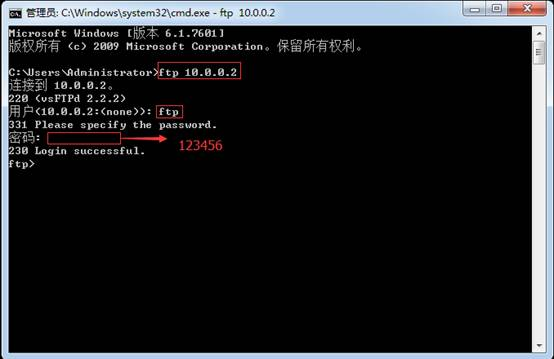
\includegraphics[width=0.40\textwidth]{2_6_1.jpeg}
  \end{center}
\end{figure}

打开 Windows server 2003 的 cmd,
输入
\begin{minted}[bgcolor=bg,breaklines=true]{sh}
ftp 10.0.0.2
\end{minted}
输入用户名 \texttt{ftp},
密码 \texttt{123456},登录成功。
\begin{figure}[H]
  \begin{center}
    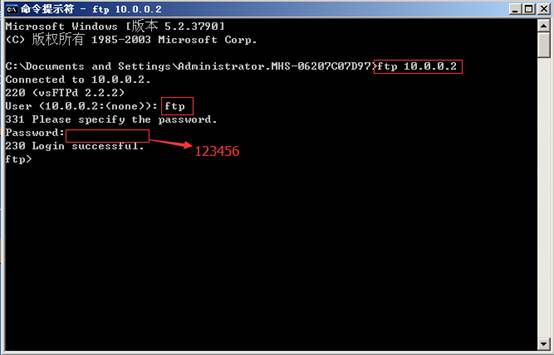
\includegraphics[width=0.40\textwidth]{2_6_2.jpeg}
  \end{center}
\end{figure}
%
\subsubsection{配置 iptables ,禁止内外网访问 ftp 服务}
在防火墙 CentOS 6.5 的终端输入如下命令,清空防火墙规则。
\begin{minted}[bgcolor=bg,breaklines=true]{sh}
iptables -F
iptables -X
iptables -Z
iptables -L -n --line-numbers
\end{minted}
\begin{figure}[H]
  \begin{center}
    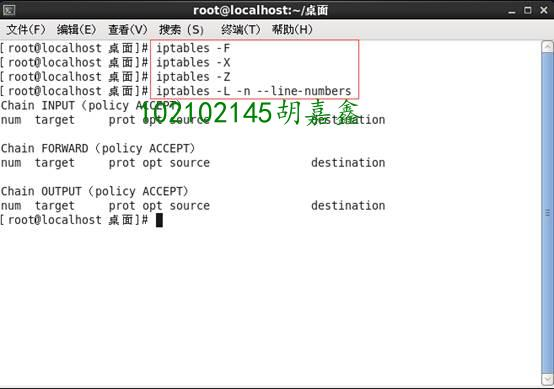
\includegraphics[width=0.40\textwidth]{2_6_3.jpeg}
  \end{center}
\end{figure}

配置防火墙,禁止内外网访问 ftp 服务。
因为这里我们使用 CentOS 6.5 充当防火墙,数据会在网卡之间进行转发,
所以我们这里对 filter 表的链 FORWARD 进行配置。
在终端输入如下命令,在转发的数据包中,如果目标端口为 21,则
将该数据包丢弃。
\begin{minted}[bgcolor=bg,breaklines=true]{sh}
iptables -t filter -A FORWARD -p tcp --dport 21 -j DROP
\end{minted}
\begin{figure}[H]
  \begin{center}
    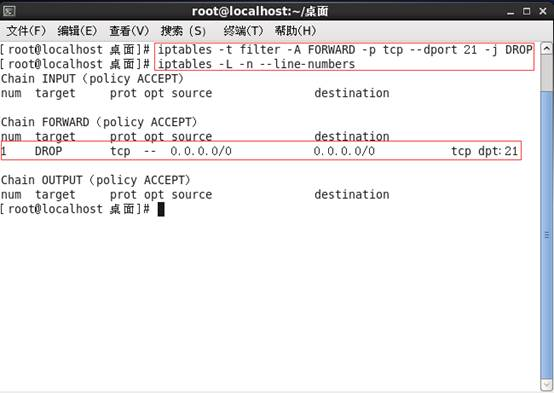
\includegraphics[width=0.40\textwidth]{2_6_4.jpeg}
  \end{center}
\end{figure}

在终端输入如下命令,将添加的规则保存到 iptables 配置文件中,重启防火墙,
查看防火墙规则。
\begin{figure}[H]
  \begin{center}
    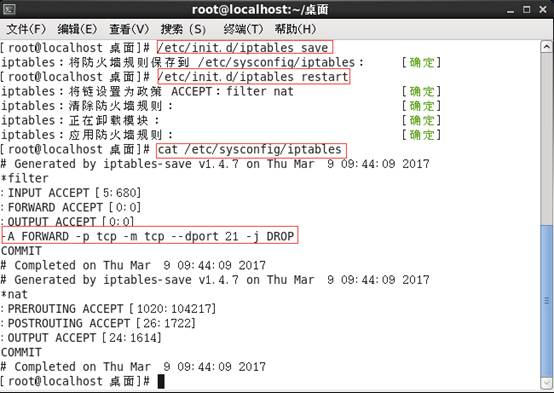
\includegraphics[width=0.40\textwidth]{2_6_5.jpeg}
  \end{center}
\end{figure}

此时在 Windows 7 的 cmd 上,输入
\begin{minted}[bgcolor=bg,breaklines=true]{sh}
ftp 10.0.0.2
\end{minted}
已经不能连接 ftp 服务了。
\begin{figure}[H]
  \begin{center}
    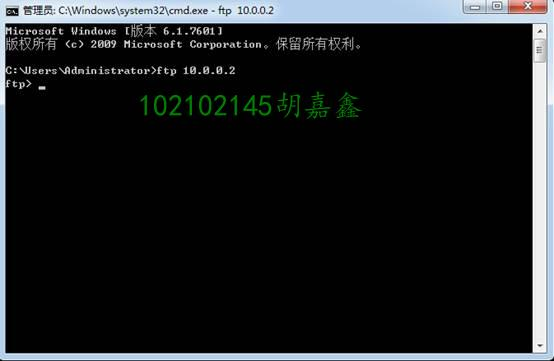
\includegraphics[width=0.40\textwidth]{2_6_6.jpeg}
  \end{center}
\end{figure}

同样在 Windows server 2003 的 cmd 上,输入
\begin{minted}[bgcolor=bg,breaklines=true]{sh}
ftp 10.0.0.2
\end{minted}
也已经不能连接 ftp 服务了。
\begin{figure}[H]
  \begin{center}
    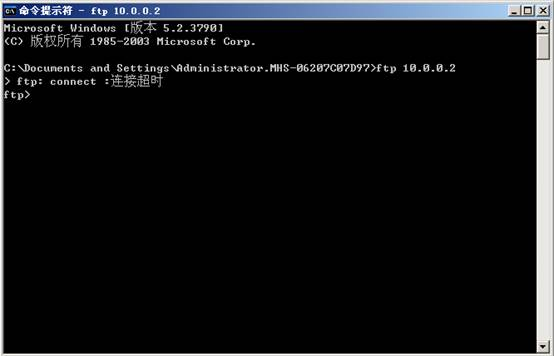
\includegraphics[width=0.40\textwidth]{2_6_7.jpeg}
  \end{center}
\end{figure}
%
